\section{Price analysis}\label{Sec:Price analysis}

One of the mean factors in the choice of the property to book is its price. Therefore one may want to try and see what other attributes influence its value.

We start in subsection \ref{subsec:corr} by calculating the correlation of all the other variables with respect to price. Then we try in subsection \ref{subsec:lm} to run a linear regression on price to look what variables are statistically relevant and how much they affect the price.


\subsection{Correlation with price}\label{subsec:corr}


Since we are only interested in the correlation with price, a normal correlation plot like the one in figure \ref{figure:corrplot} may not be the most easily readable in this case, especially because of the large number of variables.

-- UNDERSTAND HOW TO PUT IMAGE embedded in text

\begin{figure}[H]
\begin{center}
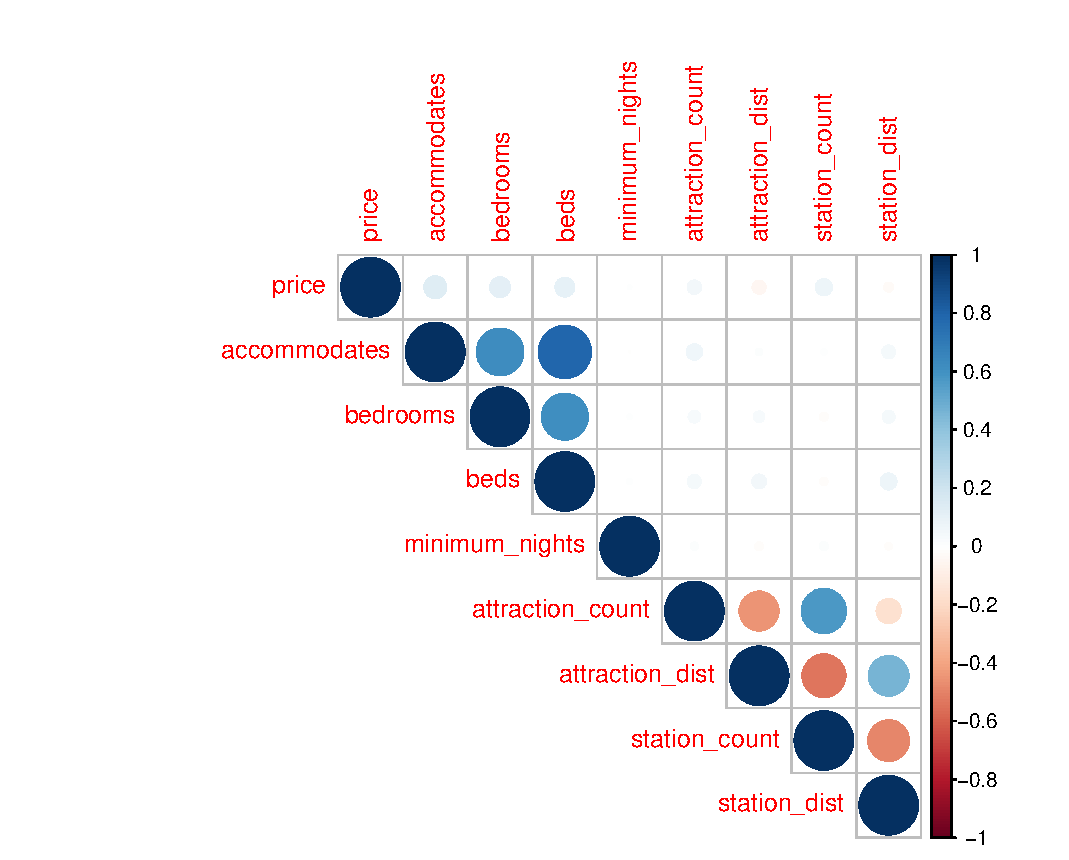
\includegraphics[width=0.5\textwidth]{corrplot.pdf}
\caption{Correlation plot with the function  \textit{corrplot} from the package \textit{corrplot} }
\label{figure:corrplot}
\end{center}
\end{figure}

In fact, categorical variables firstly need to be transformed into many dummy variables in order to calculate the correlation.




\begin{figure}[H]
\begin{center}
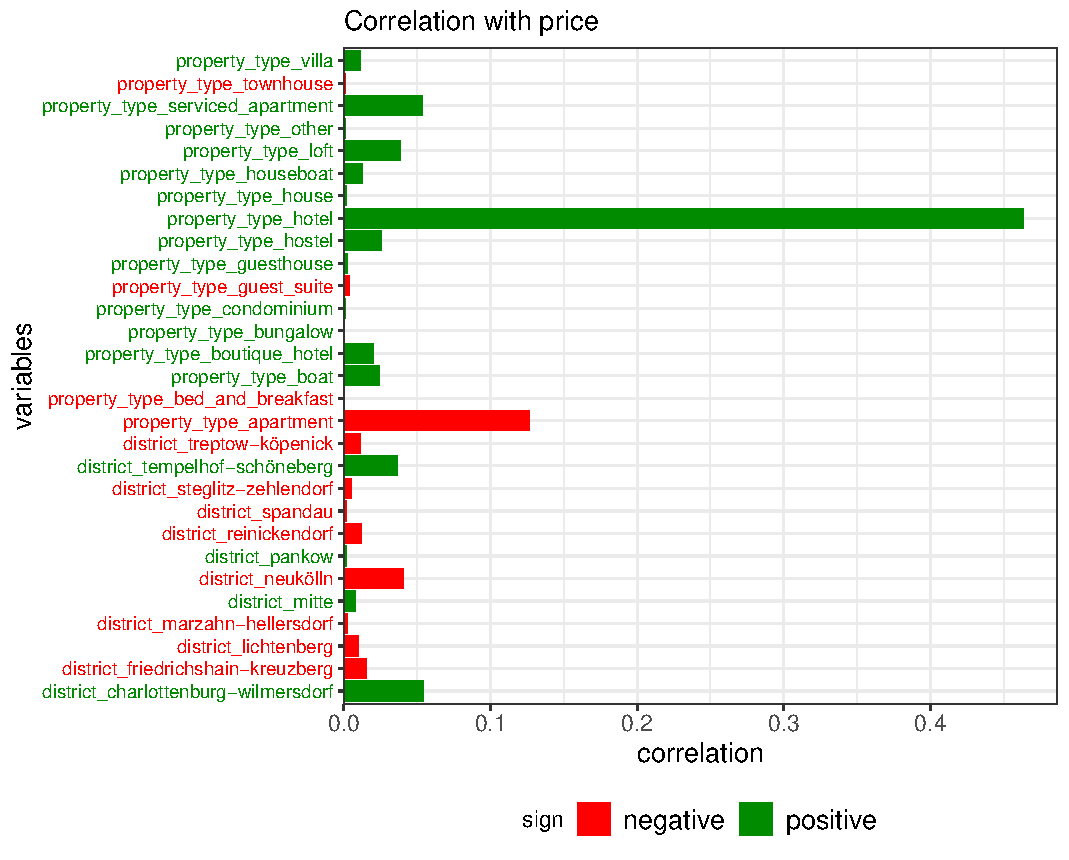
\includegraphics[width=0.8\textwidth, keepaspectratio]{price_correlation.pdf} \\
\caption{Plot of correlation with price}
\label{figure:room_type}
\end{center}
\end{figure}



\subsection{Linear regression on price}\label{subsec:lm}


